\section{Software}
\label{sec:chapterexample}
Die Hardware ist nun vollständig und dient als Basis für die Entwicklung der Softwarekomponenten die für das System notwendig sind. 
\subsection{Programmiersprachen}
Das System besteht aus mehrere Programme und Dienste. Für die Entwicklung werden folgende Programmiersprachen eingesetzt:
\begin{itemize}
	\item Java
	\item Javascript
	\item \gls{php}
\end{itemize}
Im Verbindung mit \gls{php} kommt natürlich die Markup-Languages \gls{html}5/\gls{css}, welche für die graphische Darstellung der Webapplikationen notwendig ist.

\subsubsection{Java}
\label{kap:java}
Alle Dienste die Serverseitig und ohne Interaktion mit dem Enduser ausgeführt werden, werden in Java programmiert. Als stark typisierte und Objektorientierte Programmiersprache eignet sich Java für dieses Projekt. Für Java sind auch unzählige Libraries verfügbar, insbesondere für die Hardware Steuerung der Raspberry Pi. Eine zweite Variante wäre Python gewesen, die auch das Raspberry sehr gut unterstüzt. Python ist aber zu wenig typisiert und für eher kleinere Softwarestücke gedacht.

\subsubsection{PHP/Javascript}
Die \gls{clientapp} sowohl auch die Applikation bei der \gls{aussensprechstelle} werden Web-Applikationen sein. Dies ermöglicht eine schnelle und zeitgemässe Softwareentwicklung. Für dieses Projekt ist die System-Eingriffstiefe von Webapplikationen jedenfalls ausreichend. Es muss lediglich Zugriff auf Mikrofon, Lautsprecher und Kamera garantiert werden. Ein weiteres Punkt zugunsten einer Webapplikation ist die Cross-Plattform Kompatibilität.
\\
Aus diesem Grund haben wir uns für \gls{php} (Objektorientiert) im Kombination mit Javascript/\gls{html}/\gls{css} entschieden. Eine zweite Variante wäre Java EE gewesen. Java EE eignet sich aber vor allem für grosse Softwarelösungen und bietet als gesamten Framework vieles mehr als was dieses Projekt benötigt.
\\
\subsubsection{PHP Framework: Laravel}
Für die Entwicklung der Webapplikationen wird Laravel als \gls{php} Framework eingesetzt. Laravel ist ein Open-Source \gls{php} Web-Application-Framework, die sich für kleine bis zu mittelgrosse Projekte eignet. Laravel beruht auf dem Modell-View-Controller-Muster und ermöglicht eine Objektorientierte Programmierung in \gls{php}.

\subsection{System Übersicht}
Das System besteht aus mehrere Softwarekomponenten die zusammenarbeiten müssen (\seeref{fig:echosystem}). Die  Vertraulichkeit der Kommunikation zwischen den Knoten ist von \gls{tls} immer gewährleistet. Die einzelne Komponenten, sowie das Thema Sicherheit, werden in den nächsten Kapiteln genauer beschrieben.

\begin{figure}[htb!]
	\begin{center}
		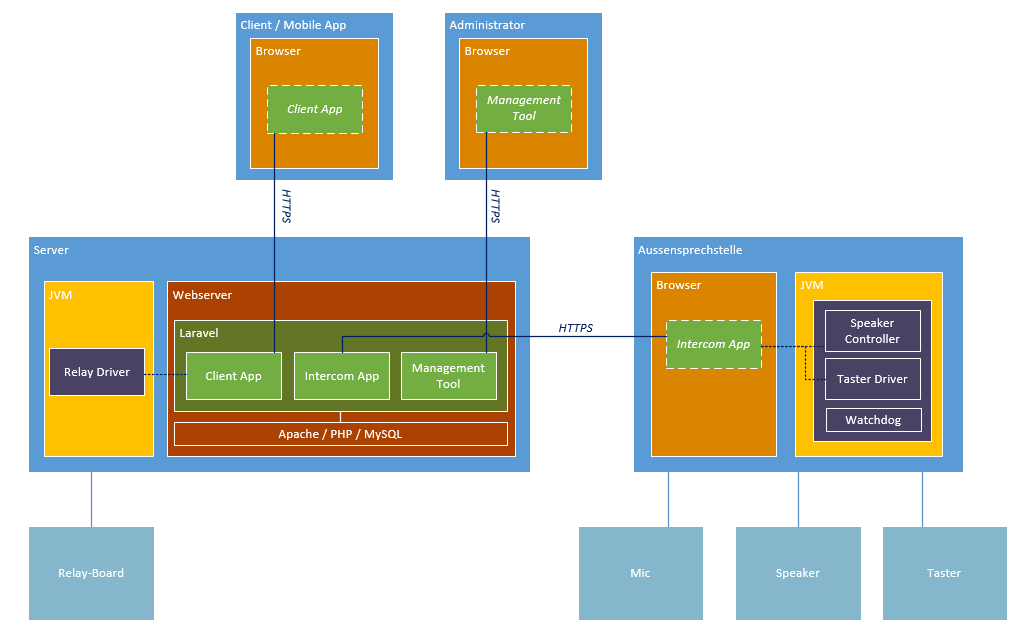
\includegraphics[width=1\textwidth]{ecosystem}
		\caption[Software Ecosystem]{Software Ecosystem}
		\label{fig:echosystem}
	\end{center}
\end{figure}

Die Software wird in zwei Gruppen unterteilt. Einerseits gibt es alle Dienste/Daemons \textit{(Violett)} die Lokal ausgeführt werden und quasi das Backend des Systems darstellen.
\\
Die zweite Gruppe beinhaltet die Webapplikationen \textit{(Grün)}, die eine \gls{gui} besitzen und für die Interaktion mit dem System gedacht sind. Darunter zählen die Client-App für den Bewohner, die Applikation bei der \gls{aussensprechstelle} wo die Bewohner angezeigt werden und das Management Tool.
\\
Die Audio/Video-Kommunikation zwischen die \gls{aussensprechstelle}n und die \gls{clientapp}en wird mithilfe von \gls{webrtc} realisiert. 

\subsection{Mühsame Security Policies}
Die Sicherheit spielt für dieses System eine grosse Rolle. Aus diesem Grund wurde von Anfang an geplant, das ganze Datenverkehr mit \gls{tls} zu verschlüsseln. Auch \gls{webrtc} selber weigert sich zu funktionieren, wenn keine gültige \gls{https} Verbindung vorhanden ist.
\\
Unglücklicherweise für die Entwicklung dieses Prototyp, sind die Security-Policies von den Heutige Browser immer mühsamer. Es ist zum Beispiel nicht mehr Möglich, den Browser so Einzustellen, dass die Zertifikat-Fehler ignoriert werden. Das hat als folge, dass auch während der Entwicklung das Zertifikat gültig und Signiert sein muss. Ansonsten funktioniert \gls{webrtc} nicht.
\\
Dies hat uns während der Entwicklung sehr viel Zeit gekostet. Zertifikate sind immer zu einem Hostname oder \gls{ip} Adresse gebunden. Das hat als folge, dass jedes mal Etwas an dem Netzwerk angepasst wurde, müssten alle Zertifikate nochmals generiert werden.
\\
Zusätzlich hat Google Chrome während der Entwicklung dieses Projekts mit der Version 58 die Security Policies geändert. Nach dem Update brauchten die Self-Signed-Certificates ein Zusätzliches Feld für das Subject Alternative Name (SAN). Im Netz war am anfang sehr wenig Hilfe zu finden und das hat nochmals viel Zeit gekostet.


\begin{quote}
	\textit{
		"[...] RFC 2818 describes two methods to match a domain name against a certificate: using the available names within the subjectAlternativeName extension, or, in the absence of a SAN extension, falling back to the commonName. The fallback to the commonName was deprecated in RFC 2818, but support remains in a number of TLS clients, often incorrectly. [...]"
	} 
	\\
	\nocite{} [ Deprecations and Removals in Chrome 58, developers.google.com ]
\end{quote}

\subsection{WebRTC}
\label{kap:webrtc}
\gls{webrtc} ist ein offener Standard, der eine Sammlung von Kommunikationsprotokollen und API beinhaltet. Die Standardisierung wird mehrheitlich betrieben und unterstützt von Google, Mozilla Foundation und Opera Software. \gls{webrtc} basiert auf \gls{html}5 und Javascript und die Audio/Video Übertragung erfolgt über eine direkte Verbindung zwischen den Sprechpartner (Peer-to-Peer).
\\
\\
\gls{webrtc} wird hauptsächlich für die Entwicklung von Videokonferenz Programme verwendet. Die Natur dieses Projekt ist allerdings nicht dieselbe wie die herkömmliche Real-Time-Communication Applikationen. Glücklicherweise wurde \gls{webrtc} so entwickelt, um möglichst viel Flexibilität zu garantieren. Aus diesem Grund beinhaltet der \gls{webrtc}-Standard keine Definition für den Signaling-Process, welcher zusammen mit dem \gls{ice} (Interactive Connectivity Establishment) für den Verbindungsaufbau zwischen den Sprechpartnern zuständig ist. 

\begin{quote}
	\textit{
		"The thinking behind \gls{webrtc} call setup has been to fully specify and control the media plane, but to leave the signaling plane up to the application as much as possible. The rationale is that different applications may prefer to use different protocols, such as the existing SIP or Jingle call signaling protocols, or something custom to the particular application, perhaps for a novel use case. [...]"
	} 
	\\
	\nocite{} [ Sam Dutton, HTML5Rocks.com ]
\end{quote}

\subsubsection{Signaling Process}
\label{kap:signaling}

Ähnlich wie bei \gls{voip}-Telefonie \textit{(\gls{sip})}, brauchen die Sprechpartner ein gemeinsam bekanntes Knoten, um die Verbindung zu initialisieren (\seeref{fig:signaling}). In den meisten Fällen ist einem Partner, die logische Adressierung der andere Partner nicht bekannt. Es besteht also keine Möglichkeit um eine \gls{p2p} Verbindung auf einmal zu starten.
\begin{figure}[htb!]
	\begin{center}
		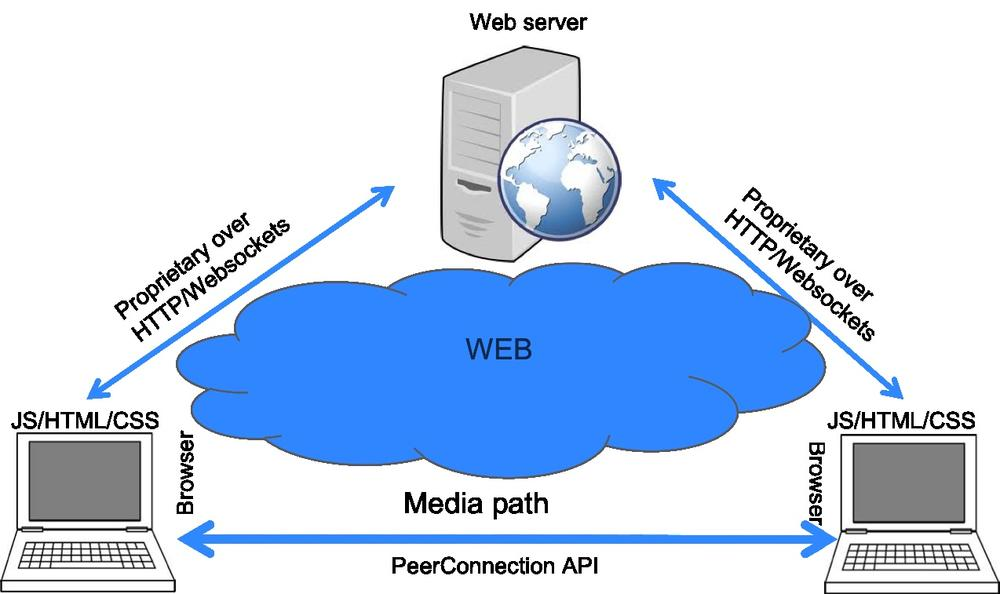
\includegraphics[width=0.75\textwidth]{signalingprocess}
		\caption[Der Signaling Prozess]{Der Signaling Prozess}
		\label{fig:signaling}
	\end{center}
\end{figure}
\\
Im unseren Fall wäre es theoretisch möglich, da die Position der \gls{aussensprechstelle} bzw. der Server immer dieselbe sind. Allerdings wurde \gls{webrtc} nicht so konzipiert. Die Standard \gls{webrtc} \gls{api} beinhaltet kein Konstrukt um eine Verbindung anhand von Bekannter \gls{ip}-Adresse aufbauen zu können.
\\
Im Internet sind es mehrere Signaling-Server Libraries verfügbar. Allerdings sind diese für andere Anwendungen gedacht. Im unseren System, wird beispielsweise nie eine Anruf von der \gls{aussensprechstelle} zu den \gls{clientapp} gestartet, sondern lediglich umgekehrt.
\\
Für die Zwecke unser Projekt wurde ein eigenes Signaling-Server entwickelt. Dieser wird auf den Server ausgeführt und somit bleibt der Datenverkehr zwischen dem \gls{clientapp} und der \gls{aussensprechstelle}, während jeder Schritt der Verbindungsaufbau und Kommunikation, innerhalb des lokales Netzwerkes. Das natürlich nur, solange der Bewohner sich zu Hause befindet.

\subsubsection{STUN Servers \& Remote Verbindung}
\label{test}
Eine Anforderung des Systems ist die Möglichkeit, auch ausserhalb des Heimnetzes mit den \gls{aussensprechstelle} sich verbinden zu können. Hier stellt das \gls{nat}-Protokoll (Network Adress Translation) ein Problem dar.
\\
Nach dem Signaling-Prozess wird das \gls{ice}-Prozess gestartet. Hier tauschen sich die zwei Partner Informationen über die eigene Adressierung und den \textit{best path} aus. Falls sich ein Sprechpartner hinter ein \gls{nat}-Knote befindet, wird für den anderen unmöglich sein eine Verbindung aufzubauen. Hier kommen die \gls{stun}-Servers im Spiel. Ähnlich wie bei dem Signalisierungsprozess stehen \gls{stun}-Servers als Hilfe für den Verbindungsaufbau da (\seeref{fig:stun}).
\begin{figure}[htb!]
	\begin{center}
		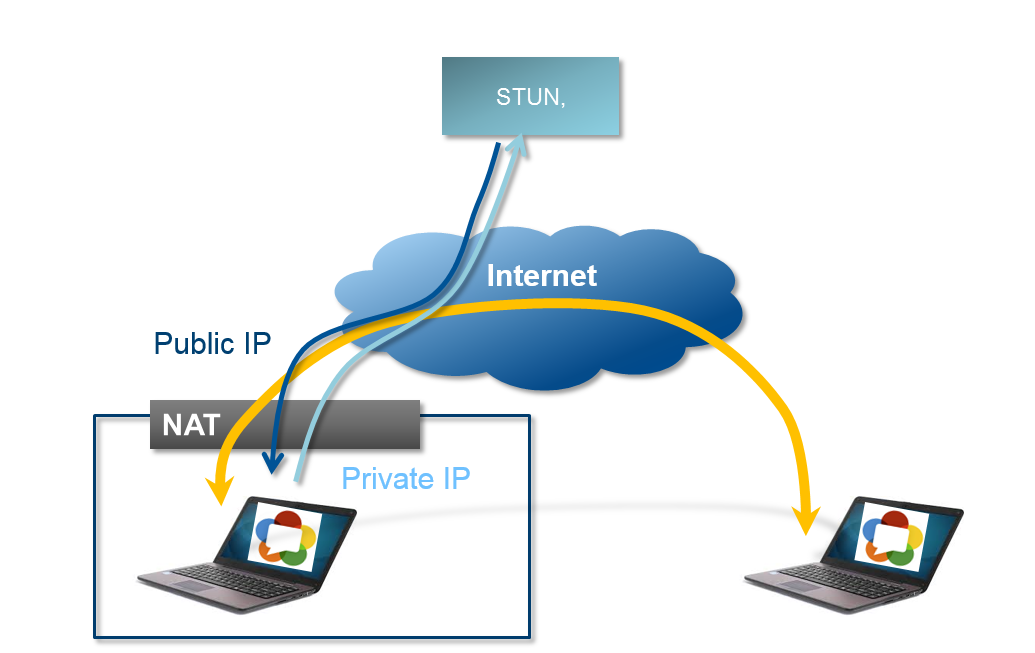
\includegraphics[width=0.75\textwidth]{stun}
		\caption[STUN Server]{STUN Server}
		\label{fig:stun}
	\end{center}
\end{figure}
\gls{stun}-Servers informieren die Clients über jegliche \gls{nat} Konfigurationen die sich dazwischen befinden würden. Die beide Sprechpartner erhalten somit Informationen über welche Ports und Öffentliche Adressen die Verbindung initialisiert werden kann. Für die Entwicklung dieses Projektes werden die Google \gls{stun} Servers verwendet, welche kostenfrei zur Verfügung stehen.
\\
Falls sich beide Sprechpartner im gleichen lokales Netzwerk befinden, werden keine \gls{stun}-Servers benötigt und den gesamten Datenverkehr bleibt innerhalb des Heimnetzwerkes.

\subsection{Webapplikationen}
\label{kap:webapp}
Während die verschiedene Java Dienste relativ kleine Programme sind, besteht den Gesamten Quellcode der Webapplikationen aus mehrere tausende Codezeilen.
\\
Das \gls{php}-Backend im Zusammenarbeit mit Javascript auf den Client-Seite ist für die meisten Aufgaben der Anlage sowohl auch für ein Teil der Sicherheitsaspekten zuständig.

\subsubsection{Client Webapplikation}
Der Bewohner muss über eine Applikation verfügen, die auf dem Tablet oder Handy ausführbar sein muss. Mithilfe dieser App muss der Enduser folgendes können: Sich mit alle \gls{aussensprechstelle}n verbinden können, ein Video Signal von der Kamera aller Eingänge erhalten, alle Türe öffnen und mit der Person bei der Türe über die Anlage kommunizieren können.
\\
\begin{figure}[htb!]
	\begin{center}
		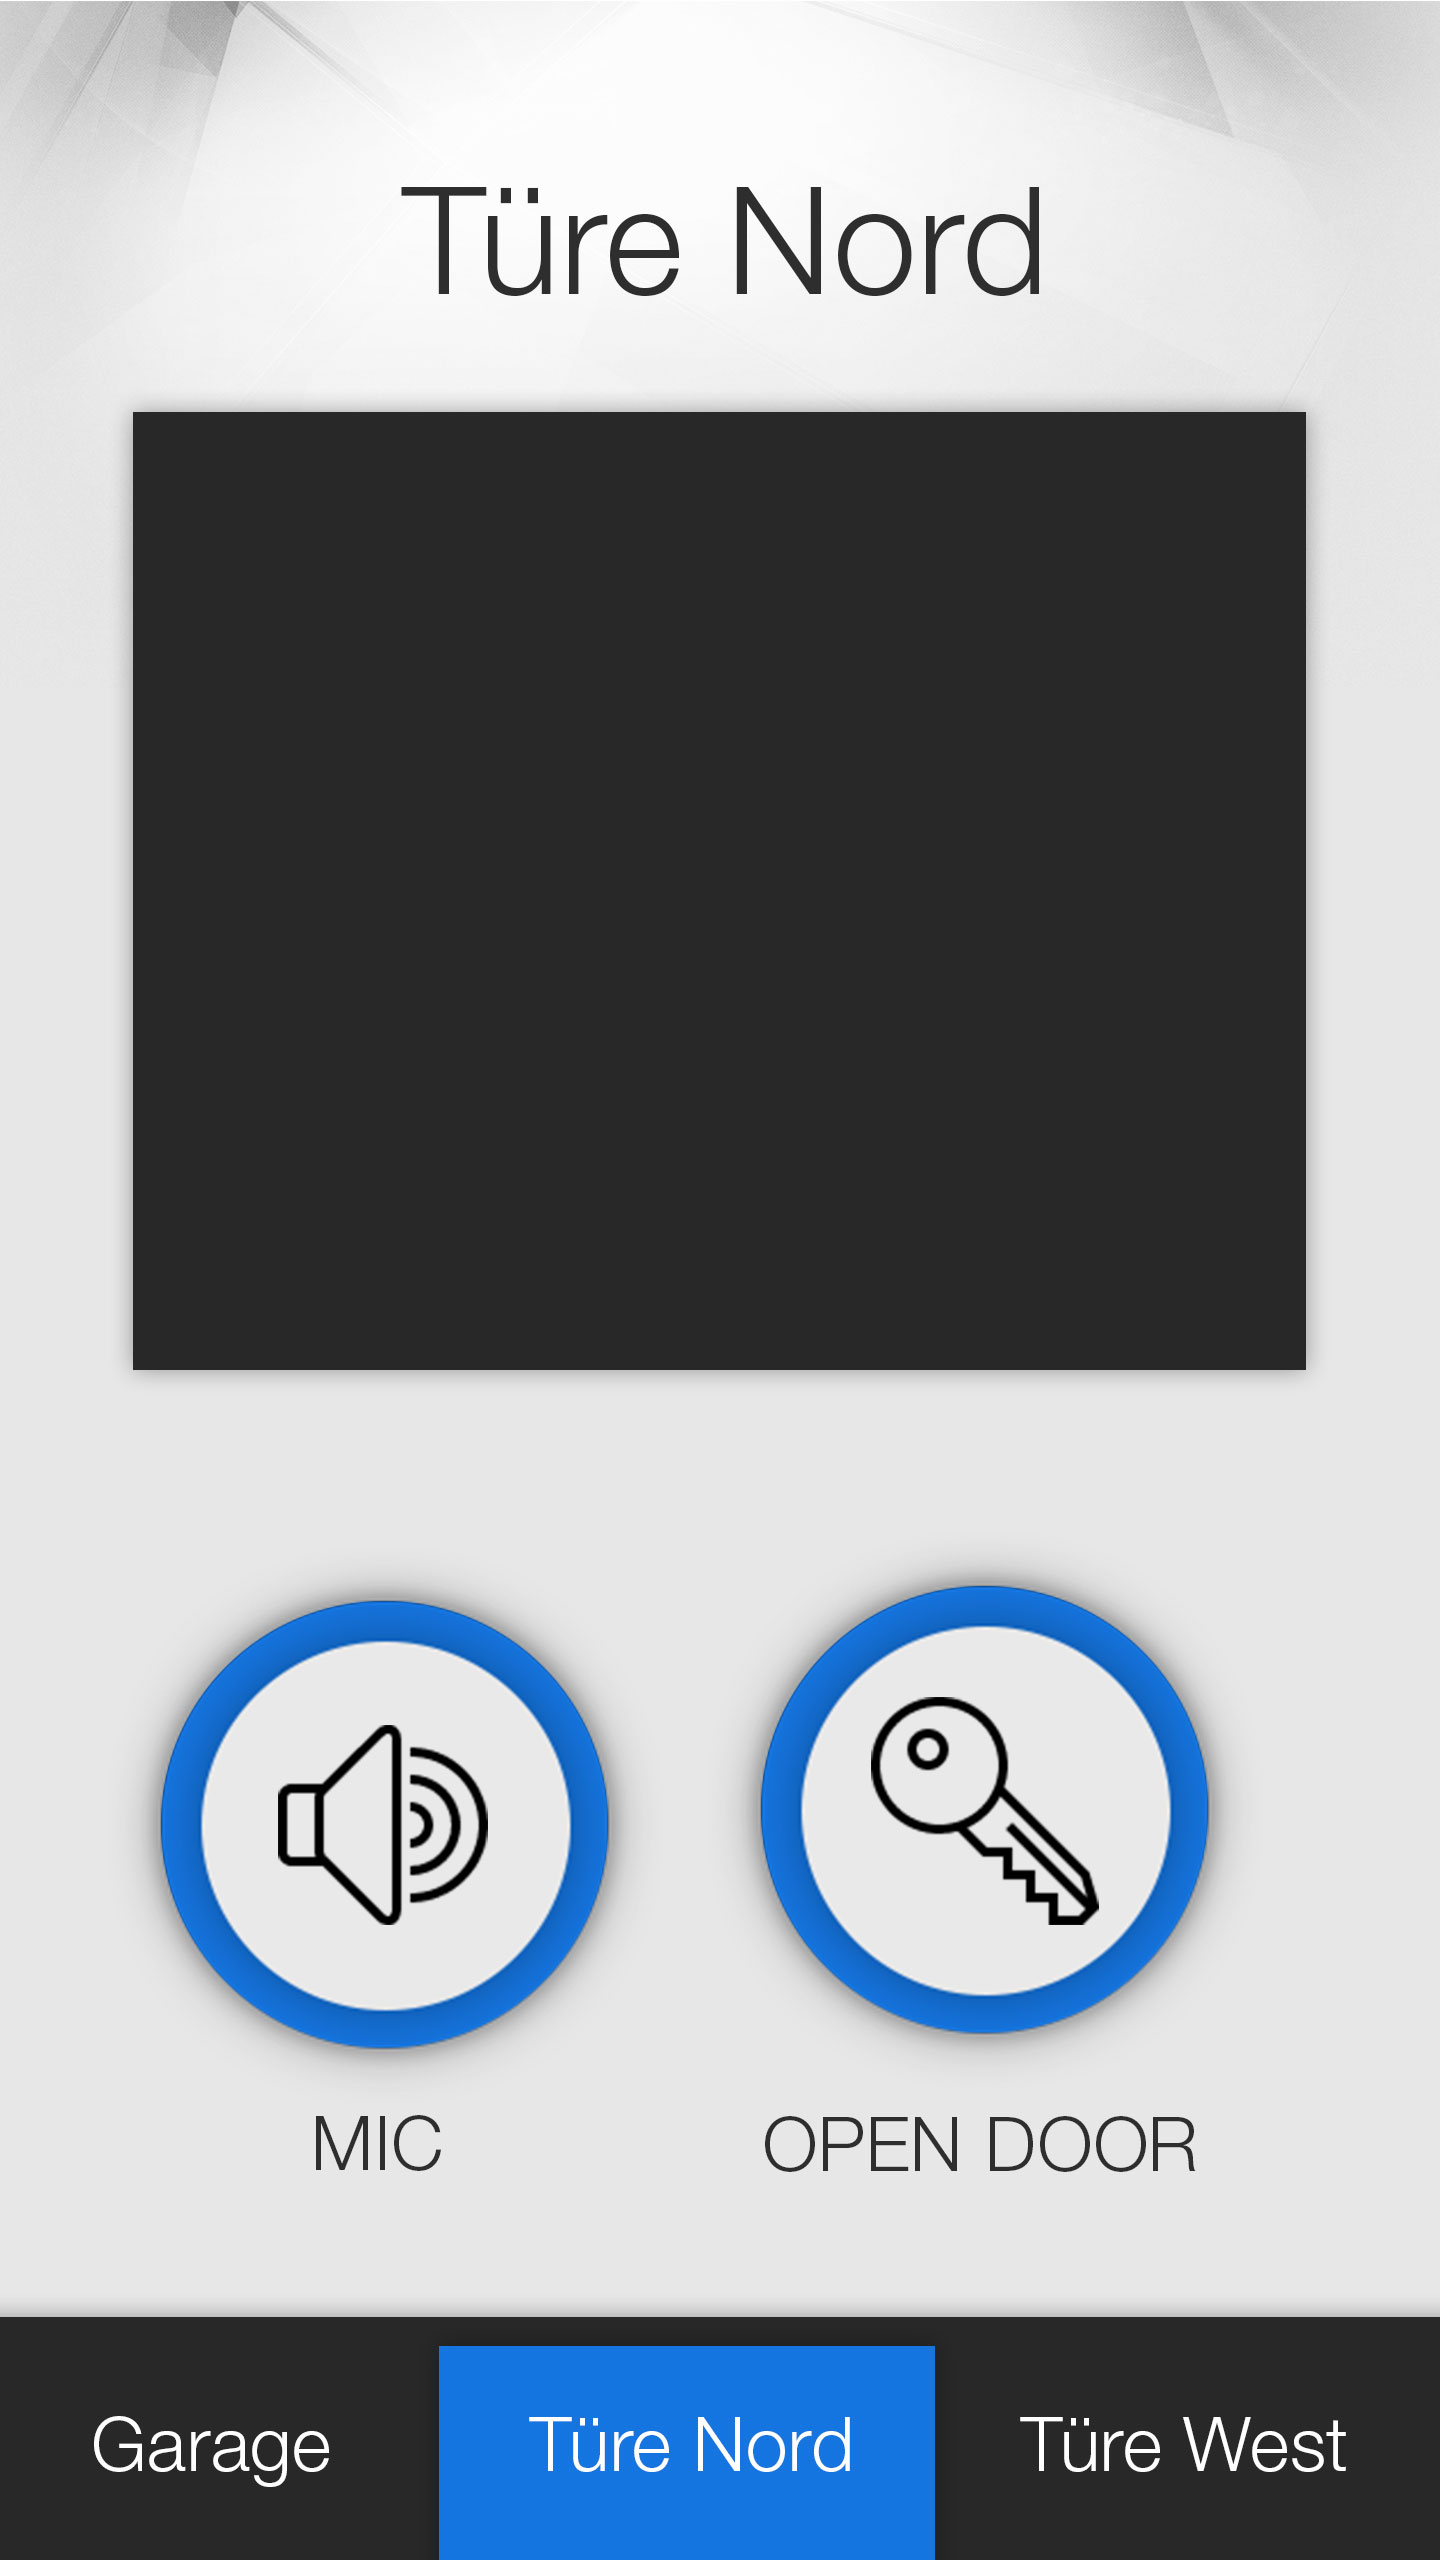
\includegraphics[width=0.35\textwidth]{clientDemo}
		\caption[Design der Client-Webapp]{Design der Client-Webapp}
		\label{fig:clientDemo}
	\end{center}
\end{figure}
\\
Die \cref{fig:clientDemo} zeigt das Design für die Webapplikation. Hier gezeigt ist die Smartphone Version. Dank ein Responsive-Design wird die selbe Applikation auch auf andere Geräte wie z.B. Tablets oder Computers passend angezeigt.
\\ 
Bei der Design-Entwurf standen Übersichtlichkeit und Benutzerfreundlichkeit im Vordergrund. Aus diesem Grund werden die Tasten für die Audio-Kommunikation und für die Öffnung der Türe gross Angezeigt. Das Videostream von der ausgewählte Türe wird sofort angezeigt und benötigt keine weitere Interaktion. 

\subsubsection{Aussensprechstelle Webapplikation}
Die \gls{aussensprechstelle} ist mit einem Bildschirm ausgestattet. Hier wird die Bewohnerliste angezeigt. Mithilfe von drei Schalter können diesen durchgeblättert und angerufen werden (\seeref{fig:doordesign}).
\\
\\
Währen der Bewohner die Möglichkeit hat, die Person an der Türe zu sehen, erhaltet der Besucher an der Türe kein Videosignal. Das wäre Technisch absolut möglich. Als Einwohner will man aber die Möglichkeit haben, die Türe nicht zu öffnen oder dem Besucher unsere Präsenz gar nicht bekanntgeben. 
\begin{figure}[htb!]
	\begin{center}
		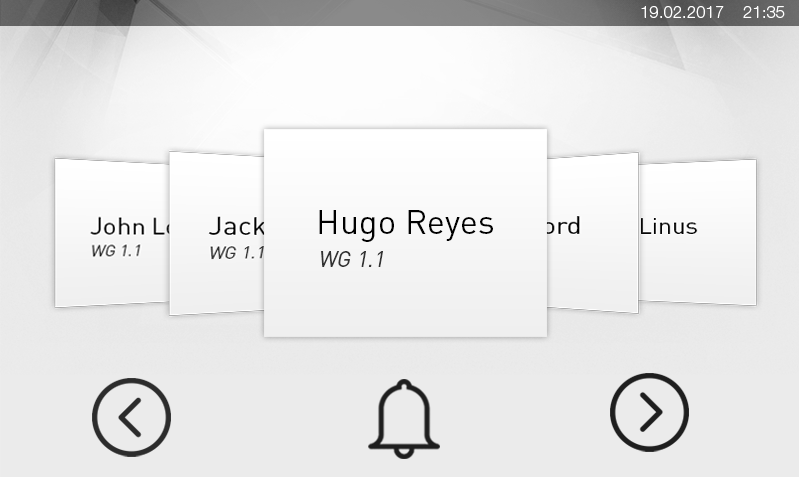
\includegraphics[width=0.70\textwidth]{doordesignbeta}
		\caption[Design der Client-Webapp]{Design der Aussensprechstelle-Webapp}
		\label{fig:doordesign}
	\end{center}
\end{figure}
\\
\\
\textbf{Probleme bei der Videoübertragung}
\\
Nach die ersten Tests der Webapplikationen ist ein weiteres Problem aufgetaucht. Die Qualität der Videoübertragung war nicht immer befriedigend. Das Problem ist aber erst aufgetaucht, nach dem Deploy der Webapplikationen auf die endgültige Hardware.
\\Nach eine Problemanalyse konnte man folgendes feststellen:
\\
\\
Für das Video encoding verwendet \gls{webrtc} das VP8 codec. Der Codierung im Gegensatz zu den Decodierung, wie bei der Mehrheit solche Systemen ist sehr Leistungsintensiv. Die \gls{aussensprechstelle} muss im Stande sein, die Codierung in Real-Time auszuführen. Das bringt die Rapspberry  an ihre Grenzen. Obwohl eine Kamera mit hohe Auflösung im Einsatz ist, wird \gls{webrtc} im Folge des niedriges Framerates die Qualität des Stream verringern. Sobald die Qualität herabgesetzt ist, ist die Raspberry wieder im Stand die Codierung im Echtzeit durchzuführen.
\\
Aufgrund der hohe Überlastung des Prozessor während der Kodierung, tauchen zusätzlich Wärmeabführung Probeme auf. Eine verlängerte Videostreaming-Session mit erhöhte Umgebungstemperaturen, könnte der Raspberry zum Absturz bringen.
\\
Der Raspberry Pi 3 war während der Entwicklungsphase des Prototyp die richtige Entscheidung. Haptgrund war der hohe Kompatibilität, die Standardisierung von ein sehr gut etabliertes Produktund, und die Stabilität. Dazu kommen noch die Unzählige Infos, Dokumentationen die im Interet über diese Microcontroller zu finden sind.
\\
\\
\textbf{Alternative}
\\ 
Mit den gesammelte Erfahrungen während der Prototyp Entwicklung kann eine bessere Alternative zur Raspberry für eine Weiterenwicklung der Anlage ausgewertet werden. 
\\
Der Microcontroller Banana Pi M3 hat in Gegensatz zum Raspberry erheblich mehr Datenverarbeitungsleistung zu bieten (\seeref{tbl:microcontrollerComparison}). Dazu kommt noch dass diese Microcontroller das \gls{h264} hardware acceleration unterstüzt und somit der Videostream weiterhin optimisiert würde.

\begin{table}[]     
	\centering
	\label{microcontrollerComparison}
	\begin{tabular}{l|ll}
		\multicolumn{1}{r|}{} & Raspberry Pi Model 3 & Banana Pi M3 \\ \hline
		CPU Cores             & 4                    & 8            \\ \hline
		CPU Design            & Cortex A53           & Cortex A7    \\ \hline
		CPU Frequenz          & 1.2GHz               & 1.8GHz       \\ \hline
		Memory                & 1GB DDR2             & 2GB DDR3     \\ \hline
		Memory Frequenz       & 400MHz               & 672MHz       \\ \hline
		H264 Decoding         & 1080P30              & 1080P60      \\ \hline
		H264 Encoding         & 1080P30              & 1080P60      \\ \hline
		Preis				  & CHF 50.0             & CHF 99.00    \\ \hline
	\end{tabular}
	\caption{Verwendete Raspberry Pi im Vegleich mit die Banana Pi Alternative}
	\label{tbl:microcontrollerComparison}
\end{table}

Ein weiteres Vorteil des Banana Pi is das der Raspbian \gls{os} ebenfalls ünterstützt wird. Die mit dem Projekt mitgeliferte Image des Betriebsistem für die \gls{aussensprechstelle}n könnte somit auf den neue Microcontroller mit geringere Aufwand aufgespielt werden. Auch die Verkabelung stellt kein Problem dar, da die Pinbelegung eins zu eins die von der Raspberry entspricht.
\\
\subsubsection{Management Tool}
\label{kap:managementtool}
Um eine schnellere Inbetriebnahme und eine zentrale Verwaltung des Systems zu gewährleisten, wurde der \gls{managementtool} etwickelt. Dieses Webapplikation ermöglicht die Erfassung von \gls{aussensprechstelle}n und Bewohnern.
Diese Schnitstelle wurde mit Webtechnologien entwickelt(\gls{html}, \gls{php}, Javascript) und wird zusammen mit den \gls{mysql} Database auf den localen Raspberry Server gehostet. Aus Sicherheitsgründen werden alle eingehende und ausgehende Verbindungen mittels \gls{tls} abhörsicher aufgebaut.
\\
Grund für das einsetzten von Webtechnologien ist die Plattformunabhängigkeit sowie die Einfachkeit und die Standardisierung der Sprachen. Für den ersten Prototyp lag der Fokus auf die funktionale Eingenschaften der Tool. Bei einer zukünfitige Weiterentwicklung des Produkt kann man, dank der Webtechnologien mit gerigere Aufwand das Tool skalieren bzw. neue Features hinzufühgen.  

\begin{figure}[htb!]
	\begin{center}
		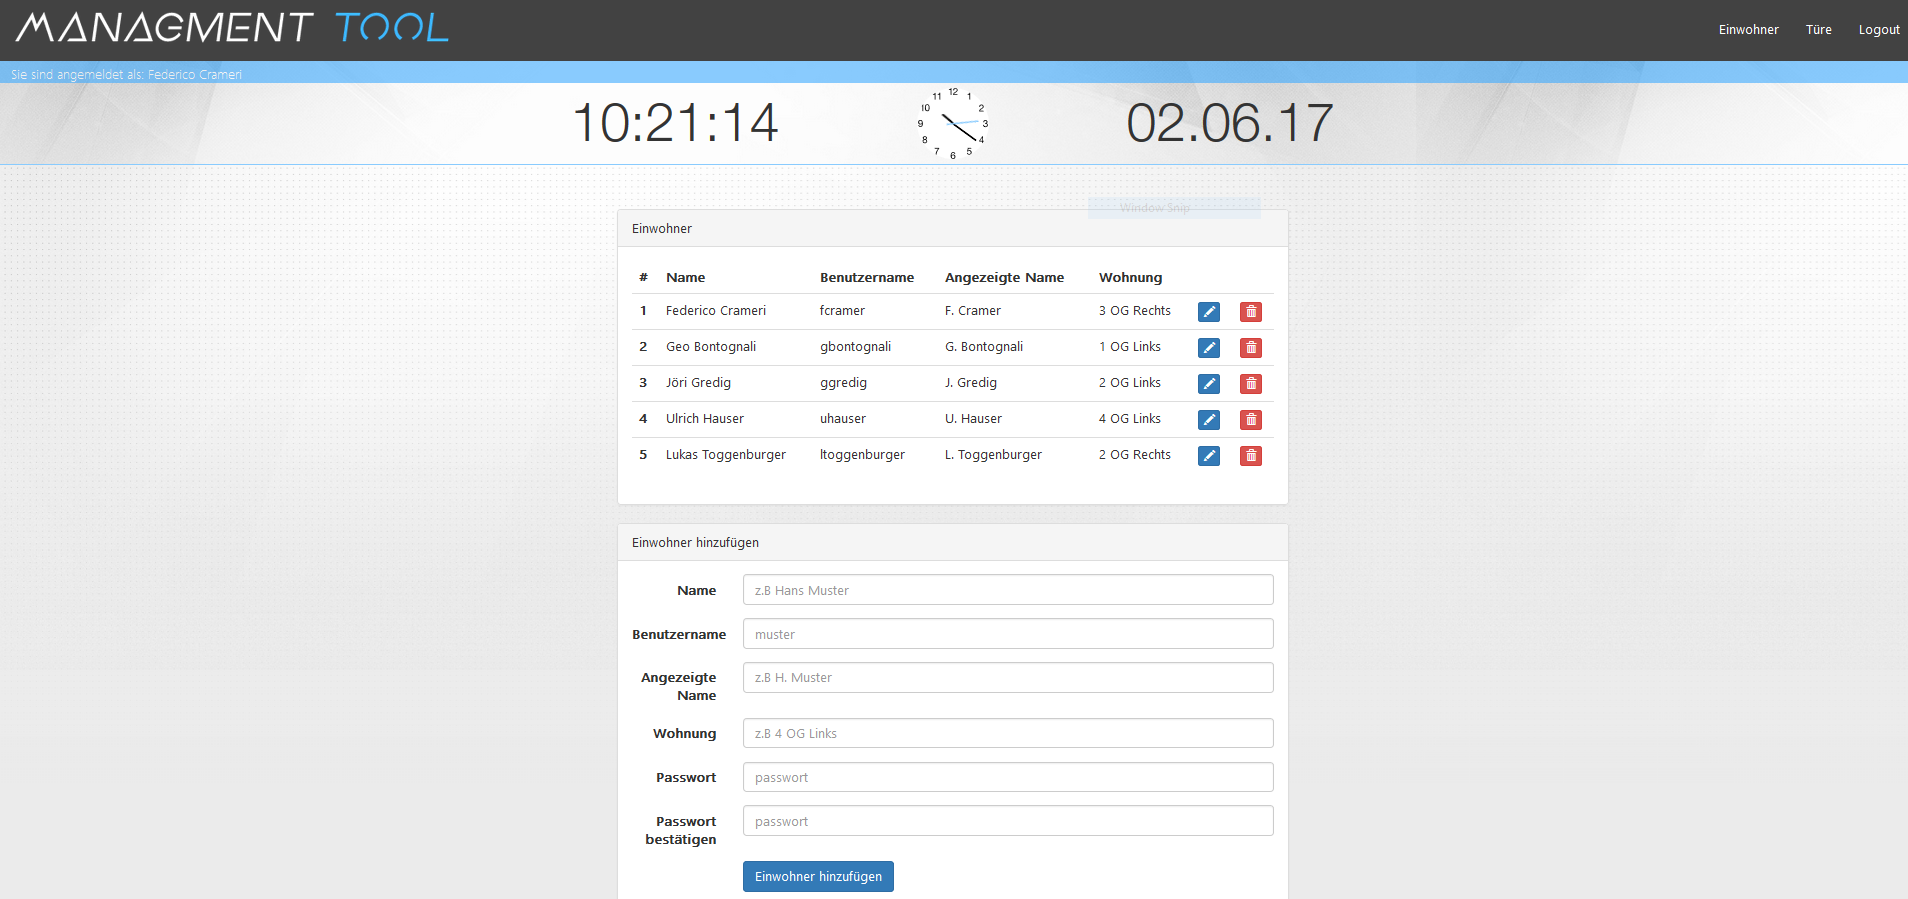
\includegraphics[width=1\textwidth]{managementtool}
		\caption[Design der Management tool]{Design der Management tool}
		\label{fig:managementtool}
	\end{center}
\end{figure}

Das Tool ist mit ein Login versehen, somit ist die Vertraulichkeit garantiert.
\\
\newline
\textbf{Bewohner} 
\\
Unter die Bewohner Seite werden alle Wohnungen, beziehungsweise alle Bewohner aufgelistet. Diese verfühgen über ein Benutzername sowie eine Passwort die von der \gls{clientapp} wervendet wird um sie sich bei den Server zu authentifizieren. Dieser Abschnitt bietet noch die Möglichkeit der Name und die Position der Wohnung welcher an den \gls{aussensprechstelle} angezeigt wird, abzuändern.
\\
\\
\textbf{Türen} 
\\
Bei der Einbau eine neue Tür, kann diese in dem \gls{managementtool} aufgeführt werden. Dabei muss beachtet werden dass der Id mit derjenige die auf den neu installierte \gls{aussensprechstelle} übereinstimmt. In diese Sektion sind auch die Namen der Türen definiert, welche denn auf den \gls{clientapp} angezeigt werden. 


\subsubsection{Remote Verbindung}
\label{kap:remote}
..


\subsection{OS und Dienste}
\label{kap:dienste}
Nun beschrieben sind alle Dienste die auf dem Raspberry laufen werden. Diese Dienste werden benötigt um die Webapplikationen mit dem Hardware zu verbinden.

\subsubsection{Raspbian}
\label{kap:raspbian}
Auf alle Raspberry Pi wurde den Betriebssystem Raspbian Jessie installiert. Diese wird von Raspberry Pi Foundation mitgeliefert und gilt als besonders hochoptimerte \gls{os} für die mit niedriger Leistung und geringem Stromverbrauch \gls{arm} Prozessoren.
Raspbian basiert auf Debian welche unter der DFSG (Debian Free Software Guidelines) Lizenz steht. Diese erlaubt der unbeschränkte Weitergabe des Software sowie abgeleitete und modifizierte  Werke weiterzugeben. 
Raspbian enthält Java SE Platform Prudukte welches und dem BCL(Oracle Binary Code License) lizensiert sind. Dieses Lizenz gewährleistet die obengenannten Freiheite ebenfalls.


\subsubsection{Taster Controller}
Die \gls{aussensprechstelle} wird durch 3 Schalter bedient. Die Aufgabe der Taster Controller besteht darin auf die \gls{gpio}s der Raspberry welcher an den Schaltern verbunden sind, abzuhöhren. Sobald ein Schalter gedrückt wird, wird eine Tastatureingabe simuliert. Durch die Simulation kann der Javascript Kode, die local im Browser ausgeführt wird, auf Schalterndruck reagieren. Somit kann auf den \gls{aussensprechstelle} Webapplikation (\seeref{fig:doordesign}) ein Bewohner ausgewählt werden (Schalter rechts und Links), und diese denn auch angerufen werden (Schalter Mitte).
\\
Die ursprüngliche Idee war das Taster Controller, so wie alle andere Dienste, als Daemon auszuführen. Das hätte den Vorteil, dass der Daemon mittels die übliche run, stop und restart Befehl gesteuert werden könnte.
Per Definition ist ein Daemon Benutzerunabhängig und genau diese Ansatzt stellte uns ein Problem dar. Eine der eingesetzten Java Library (Robot, zum Keyevent simulieren) benötigt den Zugriff auf den \gls{lxde} Desktopumgebung. Aus dem Grund das \gls{lxde} ein Benutzerspezifische Prozess ist, konnte der Taster Controller nicht als Daemon ausgeführt werden. 
\\
Um das Problem umzugehen bietet \gls{lxde} ein Autostart. Im Unix Runlevel 5 wird gewartet bis der Desktop Umgebung initialisiert ist, und erst denn wird der Taster Controller ausgeführt. Somit kann jetzt der eingesetzte Robot Library auf den \gls{lxde} zugreifen und die Tastatureingabe simulieren.  


\subsubsection{Speaker Controller}
Das Speaker Controller ist ein kleinen Dienst, welche den Lautsprecher ein- und ausschalten kann. Trotz einem Massentrennfilter sind immer noch leise Störsignale auf der Audio-Ausgang vorhanden.
Die Aufgabe des Speaker-Controllers besteht darin, die Stromspeisung des Speakers zu trennen, wenn es nicht verwendet wird. Somit ist das System Energieeffizienter und unnötige Geräusche können vermieden werden. Das Speaker Controller wird auf der \gls{aussensprechstelle} als Daemon ausgeführt.
\\
\\
Der Dienst besteht lediglich aus ein Socket-Server, der auf ein Signal wartet und durch die \gls{gpio} der Raspberry, ein kleines Relay steuert.
Das Signal kommt aus der Javascript Seite der\gls{aussensprechstelle}-Webpplikation \textit{(localhost)}. So kann den Lautsprecher bei Bedarf ein- und ausgeschaltet werden.

\subsubsection{Relay Controller}
Das Relay Controller ist sehr ähnlich aufgebaut wie das Speaker Controller. Auch hier handelt sich um ein kleines Socket-Server der auf ein Signal wartet und durch die GPIO der Raspberry, ein oder mehrere Relays steuert.
\\
Das Relay Controller wird auf dem Server ausgeführt und wartet auf die Befehle von den Webapplikationen. Das Relay ist an die Türöffner und an die Gongs in den Wohnungen angeschlossen.
\\
Der Datenaustausch zwischen den Relay-Controller und die Webapplikationen erfolgt im Form eine \gls{json} String.
\\
Währen bei der Speaker-Controller die befehle aus der Client Seite stammen, kommen die Daten bei dem Relay-Controller aus dem \gls{json}-Backend auf dem Server selbst. Somit bleibt den Datenverkehr nur auf dem Localhost und werden Man in the Middle oder Injection Attacke ausgeschlossen. Aus diesem Grund lauscht dieser Server nur auf Verbindungen die aus dem Localhost stammen.

\subsection{Logging}
\label{kap:logs}
Für die Identifikation und Rückverfolgung von Fehlern sowie für den Monitoring sind Logs File von grosse Bedeutung. Diese werden bei allen Services und Dienste konsequent druchgeführt. Das Logrotate wird nicht eingesetzt, statdessen kümmert sich das Java runtime environment um die Grösse des generiertes Log Files. Aus dem Grund dass es sich noch um ein Protoyp handelt wurde das Logging Stufe auf 7 eingestellt. In diese Stufe werden alle Emergency Nachrichten bis auf die Debug Nachrichten im Log Dateien gespeichert.
Gemäss der FHS (Filesystem Hierarchy Standard) werden die Logs unter /var/log/Aussensprechstelle gesichert. 

\subsection{Watchdog}
\label{kap:watchdog}
Die ganze Hardware, die an die Türe installiert wird, ist bei eine Endkunde schwer zugänglich. Sollte nun ein Problem mit dem System auftreten, müsste man Vorort die Anlage zurücksetzen. Die Lösung heisst hier Hardware-Watchdog, die auf dem Raspberry komplett unabhängig vom eigentlichen System läuft. Der Vorteil von ein Hardware-Watchdog ist das wenn der System bzw. der Prozessor steht, führt diese unabhängige Hardware ihre Aufgabe weiterhin aus.
Der Watchdog wird als standalone Gerät im Unix erkennt. Wird diese Gerät einmal beschrieben, dann muss diese im eine Zeitintervall von 15 Sekunden erneut beschrieben werden. Ist diese Bedingung nicht erfüllt, denn wird ein Hardware-Reset von Watchdog durchgeführt und das System wird neugestartet.
Das Beschrieben von der Watchdog-Gerät wird von eine Watchdog-Daemon übernommen. 
Durch der Konfigurationsdatei des Daemon können verschiedene Parameter des System wie Temperatur, Auslastung der Prozessor usw. überwacht werden. Besonders relevant für die Türsprechanlage ist das PID-Monitoring. Diese ermöglicht das ständig überprüfen von spezifische Prozesse und Diensten die das System benötigt, um sein Zweck als \gls{aussensprechstelle} zu erfüllen. Sobald eine diese Prozesse steht wird das System innerhalb von 15 Sekunden nuegestartet. 
Ein solches Mechanismus steigert die Verfügbarkeit des Dienst, die für eine Türsprechanlage von grosse Bedeutung ist.


\newpage